% ****** Start of file apssamp.tex ******
%
%   This file is part of the APS files in the REVTeX 4.2 distribution.
%   Version 4.2a of REVTeX, December 2014
%
%   Copyright (c) 2014 The American Physical Society.
%
%   See the REVTeX 4 README file for restrictions and more information.
%
% TeX'ing this file requires that you have AMS-LaTeX 2.0 installed
% as well as the rest of the prerequisites for REVTeX 4.2
%
% See the REVTeX 4 README file
% It also requires running BibTeX. The commands are as follows:
%
%  1)  latex apssamp.tex
%  2)  bibtex apssamp
%  3)  latex apssamp.tex
%  4)  latex apssamp.tex
%
\documentclass[%
  reprint,
  superscriptaddress,
%groupedaddress,
%unsortedaddress,
%runinaddress,
%frontmatterverbose,
%preprint,
%preprintnumbers,
%nofootinbib,
%nobibnotes,
%bibnotes,
  amsmath,amssymb,
  aps,
  prapplied,
%pra,
%prb,
%rmp,
%prstab,
%prstper,
%floatfix,
]{revtex4-2}

\usepackage{graphicx}% Include figure files
\usepackage{dcolumn}% Align table columns on decimal point
\usepackage{bm}% bold math
\usepackage{hyperref}% add hypertext capabilities
\hypersetup{
  colorlinks=true, % Set 'true' to enable colored links
  linkcolor=black, % Color of internal links (sections, pages, etc.)
  citecolor=black, % Color of citations
  filecolor=black, % Color of file links
  urlcolor=black, % Color of URL links
}
\usepackage{svg}
\usepackage{epstopdf}
\usepackage[utf8]{inputenc}
\usepackage[T1]{fontenc}
\usepackage{amsmath}
\usepackage{amsfonts}
\usepackage{amssymb}
%\usepackage[mathlines]{lineno}% Enable numbering of text and display math
%\linenumbers\relax % Commence numbering lines

%\usepackage[showframe,%Uncomment any one of the following lines to test
%%scale=0.7, marginratio={1:1, 2:3}, ignoreall,% default settings
%%text={7in,10in},centering,
%%margin=1.5in,
%%total={6.5in,8.75in}, top=1.2in, left=0.9in, includefoot,
%%height=10in,a5paper,hmargin={3cm,0.8in},
%]{geometry}
\usepackage{lipsum}

\begin{document}

\preprint{APS/123-QED}

\title{A coherently stimulated Brillouin spectrometer}

\author{Joel N. Johnson}
  \email{joel.johnson@nau.edu}
  \affiliation{Department of Applied Physics and Materials Science, Northern Arizona University, Flagstaff, AZ, 86011, USA}
  \affiliation{Center for Materials Interfaces in Research and Applications, Northern Arizona University, Flagstaff, AZ, 86011, USA}

\author{Peter T. Rakich}
  \affiliation{Department of Applied Physics, Yale University, New Haven, CT, 06520, USA}

\author{Co Authors}
  \affiliation{Department, Address}

\author{Ryan O. Behunin}
  \email{ryan.behunin@nau.edu}
  \affiliation{Department of Applied Physics and Materials Science, Northern Arizona University, Flagstaff, AZ, 86011, USA}
  \affiliation{Center for Materials Interfaces in Research and Applications, Northern Arizona University, Flagstaff, AZ, 86011, USA}

\date{\today}

\begin{abstract}
ALorem ipsum dolor sit amet, consectetur adipiscing elit. Nulla eget dolor at diam volutpat congue sit amet non magna. Phasellus sed ante ornare, commodo elit id, euismod enim. Mauris posuere, erat id vehicula ultrices, erat nisi faucibus lorem, at vehicula enim orci in dui. Nulla facilisi. Integer sed tortor venenatis, aliquet nulla quis, fermentum libero. Proin sit amet metus nec ante fermentum gravida at nec odio. Praesent id nisi ut sapien rutrum hendrerit. Donec vel sapien et eros accumsan tempus. Maecenas non velit nec nulla cursus faucibus sit amet sed dui. Ut eleifend, magna in fermentum efficitur, ligula ipsum blandit libero, sed iaculis eros magna ut arcu. Fusce eget lectus aliquet, consequat dolor at, aliquam urna. Curabitur pharetra, arcu sed vehicula maximus, nibh leo sollicitudin elit, vitae dapibus odio metus gravida ante. Aliquam erat volutpat. Donec venenatis erat vel ultrices suscipit. Nulla consequat massa quis enim. Donec pede justo, fringilla vel, aliquet nec, vulputate eget, arcu. In enim justo, rhoncus ut, imperdiet a, venenatis vitae, justo.

%\begin{description}
%\item[Usage]
%Secondary publications and information retrieval purposes.
%\item[Structure]
%You may use the \texttt{description} environment to structure your abstract;
%use the optional argument of the \verb+\item+ command to give the category of each item.
%\end{description}
\end{abstract}

\keywords{Brillouin scattering, phonon spectrometer, photonics, femtowatt, pump-probe, instrument, room-temperture, nano-acousto-optic devices}%Use showkeys class option if keyword display desired

\maketitle

%\tableofcontents


\section{Introduction}
\label{sec:Introduction}

Brillouin scattering is the inelastic scattering of light from acoustic phonons. Spontaneous Brillouin scattering is light scattering specifically with the thermodynamic fluctuations in a material. Sufficient optical power elevates this spontaneous process into stimulated Brillouin scattering: a regime in which the optical fields augment the optical properties of the material, greatly enhancing the optomechanical response. This occurs as the backscattered (e.g. Stokes) light beats with the incident pump light to induce an electrostrictive modulation that reinforces the acoustic phonons in the material. It would be desirable to introduce a high-powered fourth optical field dedicated to electrostrictive reinforcement, further stimulating the acoustic field, however phase matching conditions require that its frequency and wavevector be identical to that of the backscattered light, preventing distinguishability.

In this work, we present a coherently stimulated Brillouin spectrometer that utilizes a detuned pump-probe design to perform traveling-wave phonon spectroscopy at scales previously unachievable with traditional stimulated Brillouin techniques. With this method, we achieve sub-10 femtowatt sensitivity and enable room temperature traveling-wave phonon spectroscopy at the micrometer scale. We demonstrate the capabilities of the instrument by observing Brillouin scattering at room temperature in 1 centimeter of UHNA3 fiber and 100 micrometers of bulk carbon disulfide liquid. This instrument opens the door to nanometer-scale Brillouin spectroscopy with usage of higher optical powers and enables the characterization and development of novel nano-acousto-optic devices.


\section{Theoretical Framework}
\label{Theoretical Framework}

\subsection*{Coherently stimulated four-wave Brillouin scattering}
\label{Theoretical Framework:Coherently stimulated five-wave Brillouin scattering}
Stimulated Brillouin scattering, illustrated by the schematic in Fig. \ref{fig:4-Wave-Brillouin-Scattering}(a) for the Stokes process, is a three-wave mixing process in which incident pump laser light of frequency $\omega_{Pump}$ inelastically scatters from a traveling-wave phonon of frequency $\Omega$ to produce light that is frequency-shifted by the phonon frequency. In the Stokes process the phonon is retreating from the incident laser light and the scattered light is shifted down in frequency ($\omega_{Stokes} = \omega_{Pump} - \Omega$). Light scattered in the backwards direction spatially overlaps with the incident laser light, allowing the two optical fields interfere to produce a frequency at the difference between the two ($\omega_{Pump} - \omega_{Stokes}$). Since this difference frequency is exactly equal to the frequency of the acoustic field $\Omega$, the beating of the incident pump light and the backscattered Stokes light produces an electrostrictive reinforcement of the acoustic wave. This driving of the acoustic wave in turn increases the scattering rate of the incident pump light, producing a positive feedback process and an exponential increase of the amplitude of the backscattered Stokes wave.

\begin{figure*}[t]
  \centering
  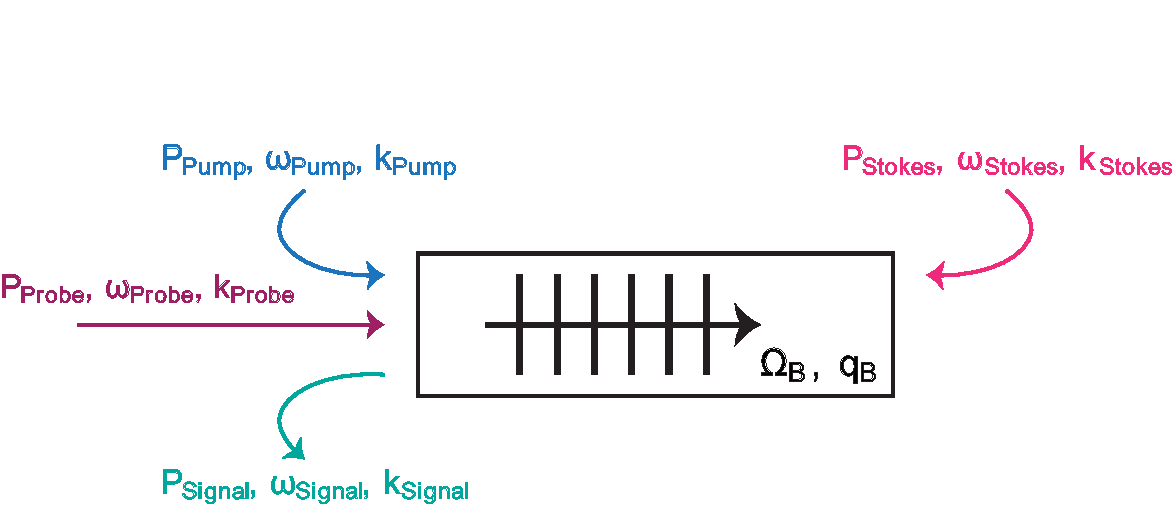
\includegraphics[width=.5\textwidth]{4-Wave-Brillouin-Scattering.pdf}
  \caption{Illustration of 4-Wave Brillouin Scattering.}
  \label{fig:4-Wave-Brillouin-Scattering}
\end{figure*}

Fig. \ref{fig:4-Wave-Brillouin-Scattering}(b) shows the schematic of coherently stimulated four-wave Brillouin scattering for the Stokes process. We introduce a dedicated external Stokes laser of frequency $\omega_{Stokes}$ that strongly drives the electrostrictive reinforcement of the acoustic field in the material. The backscattered Stokes light which is normally collected in an SBS process to infer mechanical properties of the material is now drowned out by the much higher power external Stokes laser. To resolve this, we introduce an additional external laser at a distinct frequency $\omega_{Probe}$ which copropagates with the pump laser and backscatters in the material from the strongly driven acoustic field. This produces a backscattered signal to be collected ($\omega_{Signal} = \omega_{Probe} - \Omega$) which is distinguishable from the high-powered Stokes laser light.

A full derivation of the coupled-wave equations for this four-wave mixing process can be found in Appendix \ref{Appendix:Coupled-Wave Equations}, where the scattered power of the backscattered signal is shown to be
\\
\begin{equation}
  P_{Signal} = \frac{1}{4}(G_{B}L)^{2}P_{Pump}P_{Stokes}P_{Probe}sinc^{2}\left(\frac{\Delta kL}{2}\right),
  \label{Eq:Theoretical Framework:Scattered Power} %compress sinc term into Psi here?
\end{equation}
\\
where $G_{B}$ is the coherently stimulated Brillouin scattering gain factor,
\\
\begin{equation}
  G_{B} = g_{0}\frac{\left(\frac{\Gamma_{B}}{2}\right)^{2}}{(\Omega - \Omega_{B})^{2} + \left(\frac{\Gamma_{B}}{2}\right)^{2}},
\end{equation}
\\
with the on-resonance gain factor of the material given by
\\
\begin{equation}
  g_{0} = \left[\frac{\epsilon_{0}^{2}\omega^{2}q^{4}\gamma_{e}^{4}}{n^{2}c^{2}\rho_{0}^{2}}\right].
\end{equation}
Here, $q$ is the wavevector of the driven acoustic field, $\gamma_{e}$ is the electrostrictive constant, $n$ is the refractive index of the material, $\rho_{0}$ is the mean density of the material, $\Omega_{B}$ is the resonant Brillouin frequency of the material, $\Gamma_{B}$ is the Brillouin linewidth, or dissipation rate, of the material, and $\Delta k$ is the wavevector mismatch between the optical fields, to be discussed next.


\subsection*{Phase matching relaxation}
\label{Theoretical Framework: Phase matching relaxation}
In all nonlinear optical processes, efficiency is maximized when phase matching conditions are satisfied. A frequency mismatch (energy unconservation) or a wavevector mismatch (momentum unconservation) each result in drastically reduced efficiency of a given process.\cite{maker1962effects} This can be seen by Eq. \ref{Eq:Theoretical Framework:Scattered Power}, where the wavevector mismatch, $\Delta k$, is contained within a $sinc^{2}$ function. This $sinc^{2}$ term thereby defines the phase matching bandwidth of the system, notably scaling with effective interaction length $L$.

We apply this wavevector mismatch allowance to the pump and probe waves ($\Delta k = k_{Pump} - k_{Probe}$) so that the backscattered signal is different than the applied Stokes wave. This choice allows for selection of the signal and rejection of the Stokes with a bandpass filter. Expressed in terms of wavelengths, this gives
\\
\begin{equation}
  \Delta k = \frac{4\pi n\Delta\lambda}{\lambda_{Pump}\lambda_{Probe}} \approx \frac{4\pi n\Delta\lambda}{\lambda_{Pump}^{2}}.
\end{equation}
\\
We can apply this to the phasematching bandwidth term to find the fraction of maximum scattered power, $\Phi$, that can be expected for a given $L$ and phase mismatch $\Delta\lambda$ between the pump and probe,
\\
\begin{equation}
  \Phi \equiv sinc^{2}\left(\frac{2\pi n\Delta\lambda L}{\lambda_{Pump}^{2}}\right).
\end{equation}
\\
Using this expression for $\Phi$, we see that for an effective length of one meter a wavelength mismatch of only $0.6\,pm$ from $1.55\,\mu m$ pump light in UHNA3 fiber drops the scattered power to one half of maximum. However, for shorter effective lengths the wavevector mismatch becomes more forgiving; a $36\,pm$ mismatch preserves 82.5\% of the maximum signal for a length of $1\,cm$ and all else equal. This separation, translating to about $4.5\,GHz$, is meaningful, as it represents sufficient spectral separation for the backscattered signal to be isolated from the applied Stokes light.




\section{Methods}\label{Methods}
\subsection*{Instrument design}
\label{Methods:Instrument Design}

\begin{figure*}[t]
\centering
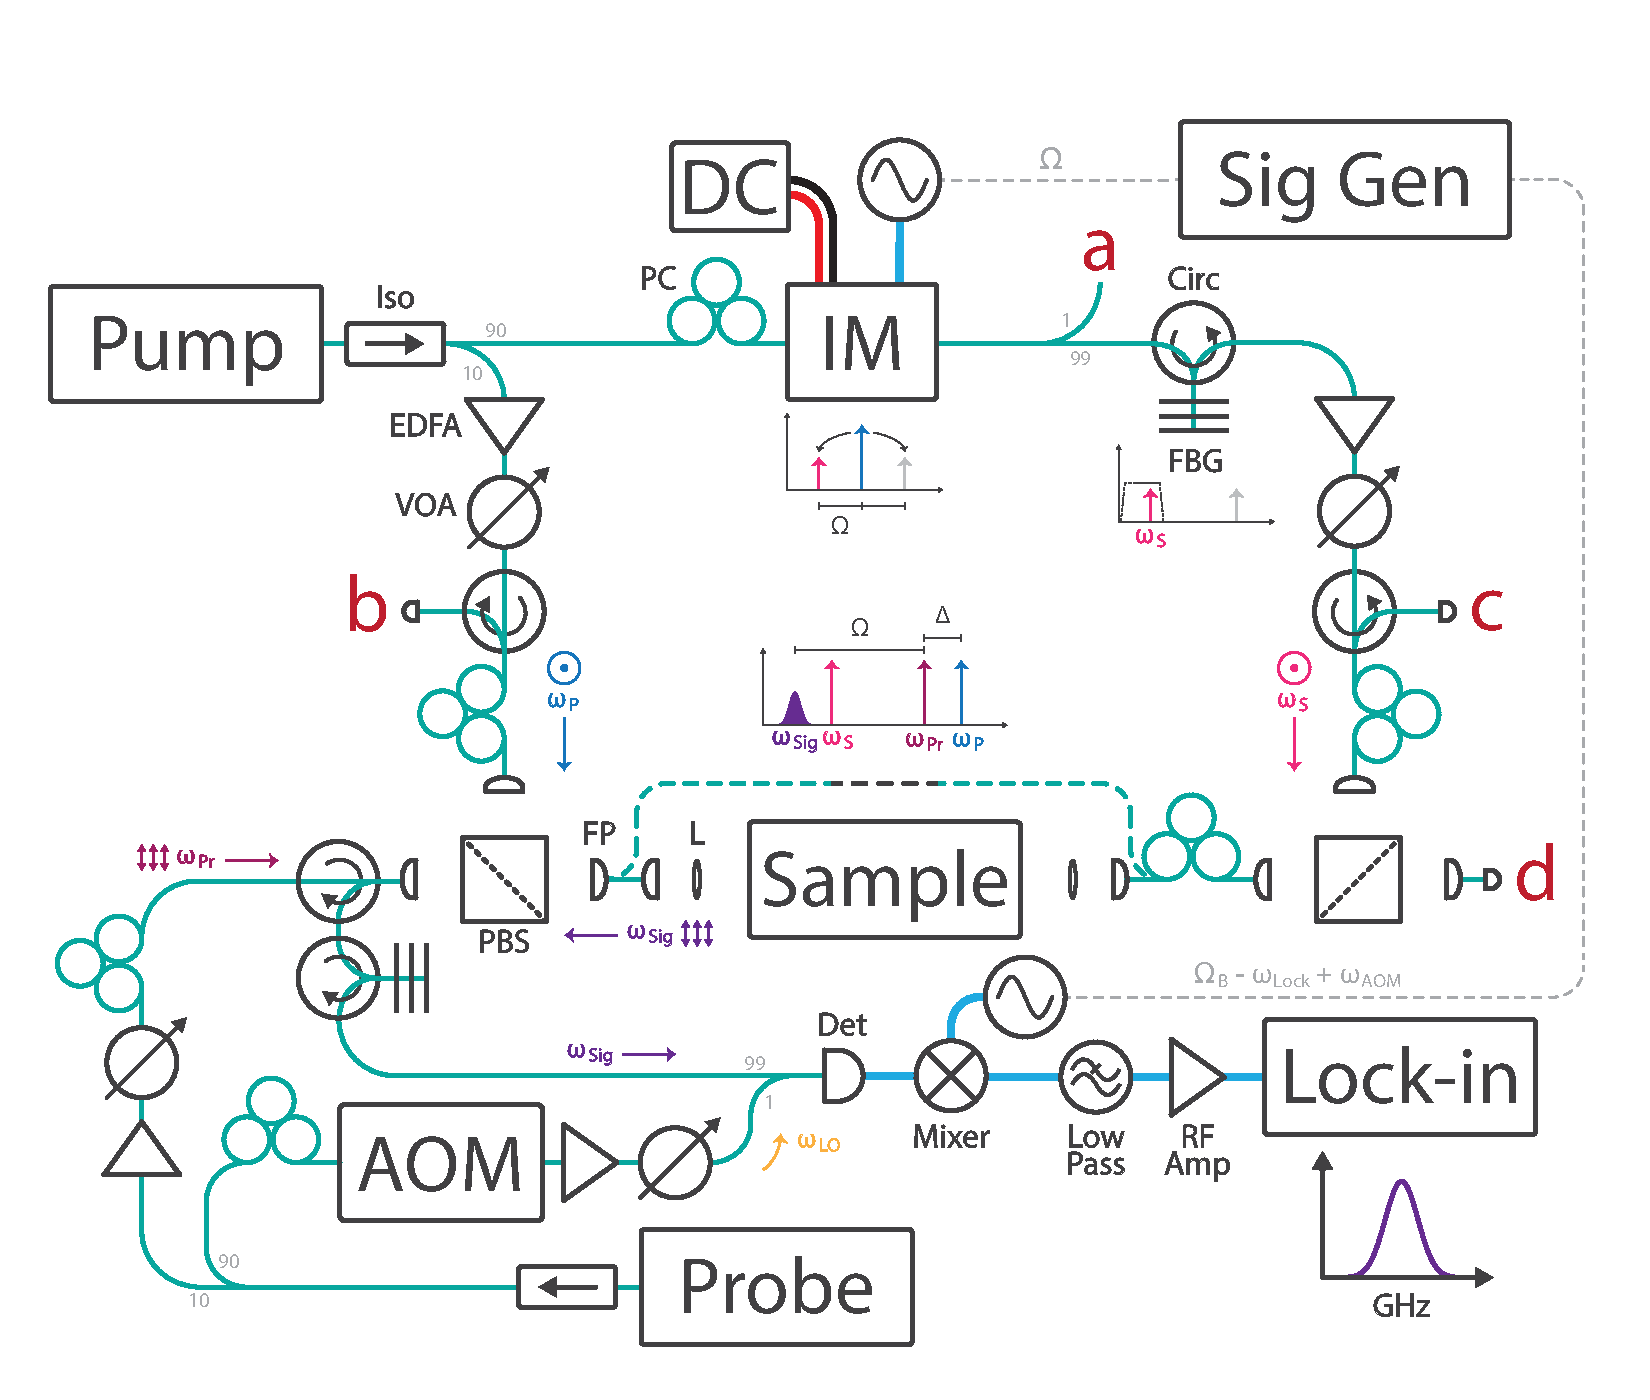
\includegraphics[width=\textwidth]{Instrument-Design-V1.pdf}
\caption{Instrument design diagram}
\label{fig:Instrument Design}
\end{figure*}

The design of the instrument is shown in the schematic in Fig. \ref{fig:Instrument Design}. A pump and Stokes signal is synthesized from a single tunable laser source for coherent stimulation of the sample. The pump signal ($\omega_{Pump}$) is amplified by an erbium-doped fiber amplifier (EDFA) and passed through a variable optical attenuator (VOA) for power control. The output is then polarization-controlled to reflect at a polarizing beam splitter (PBS) for injection into the sample. For Stokes synthesis, an AC signal ($\Omega$) is supplied to an intensity modulator with carrier frequency nulled and a tunable filter is used to select one side band output ($\omega_{Pump} - \Omega$). This Stokes light is then amplified by an EDFA, passed through a VOA, and polarization-controlled to reflect at a second PBS for couter-propagation to the pump through the sample.

A separate tunable laser ($\omega_{Probe} = \omega_{Pump} + \Delta k$) is used to synthesize the probe and local oscillator (LO). Probe light is amplified by an EDFA and fed through a VOA. A polarization controller aligns the polarization axis of the probe light for transmission through the first PBS and copropagation with the pump into the sample. Backscattered probe light exits the sample and transmits back through the first PBS, whereas the orthogonally polarized Stokes light reflects at this same point to be diverted to a tap for power monitoring. The backscattered signal ($\omega_{Signal} = \omega_{Probe} + \Omega$) then routes through two subsequent circulators for spectral filtering by a $5\,GHz$ bandpass tunable filter. This filter allows the frequency-shifted probe light to pass while rejecting (1) any reflected probe light, and (2) any reflected, transmitted, or backscattered pump or Stokes light that was not already diverted by the PBS.

The filtered signal heterodynes via a 99-1 splitter with the LO ($\omega_{LO} = \omega_{Probe} + 2\pi\times40\,MHz$), which has been frequency-upshifted by an acousto-optic modulator (AOM) and controlled to be copolarized with the backscattered signal. We consider only the subtracted frequency term of the heterodyne process as all others (original, additive, higher-harmonic, and more complicated intermodulation product frequency terms) are well beyond the range of detection. This heterodyned signal ($\omega_{signal} = \Omega + 2\pi\times40\,MHz$) is then captured by a photodiode detector and heterodyned again by a radio frequency (RF) mixer with a second AC signal ($\Omega - 2\pi\times5\,MHz$) that synchronously sweeps with the Stokes-synthesis AC signal. The resulting constant signal ($\omega_{Lock-in} = 2\pi\times45\,MHz$) is passed through a 50 MHz low-pass filter, amplified with an RF amplifier, and finally supplied to a lock-in amplifier for data collection. The lock-in amplifier is able to lock-in on the constant input frequency throughout a measurement as both AC signals, one supplied to the RF mixer and the other for Stokes synthesis, are synchronously swept through a range of frequencies during measurement.


\section{Results}\label{Results}
\subsection*{Instrument sensitivity and SBS comparison}
\label{Results:Instrument sensitivity and SBS comparison}

\begin{figure}[t]
  \centering
  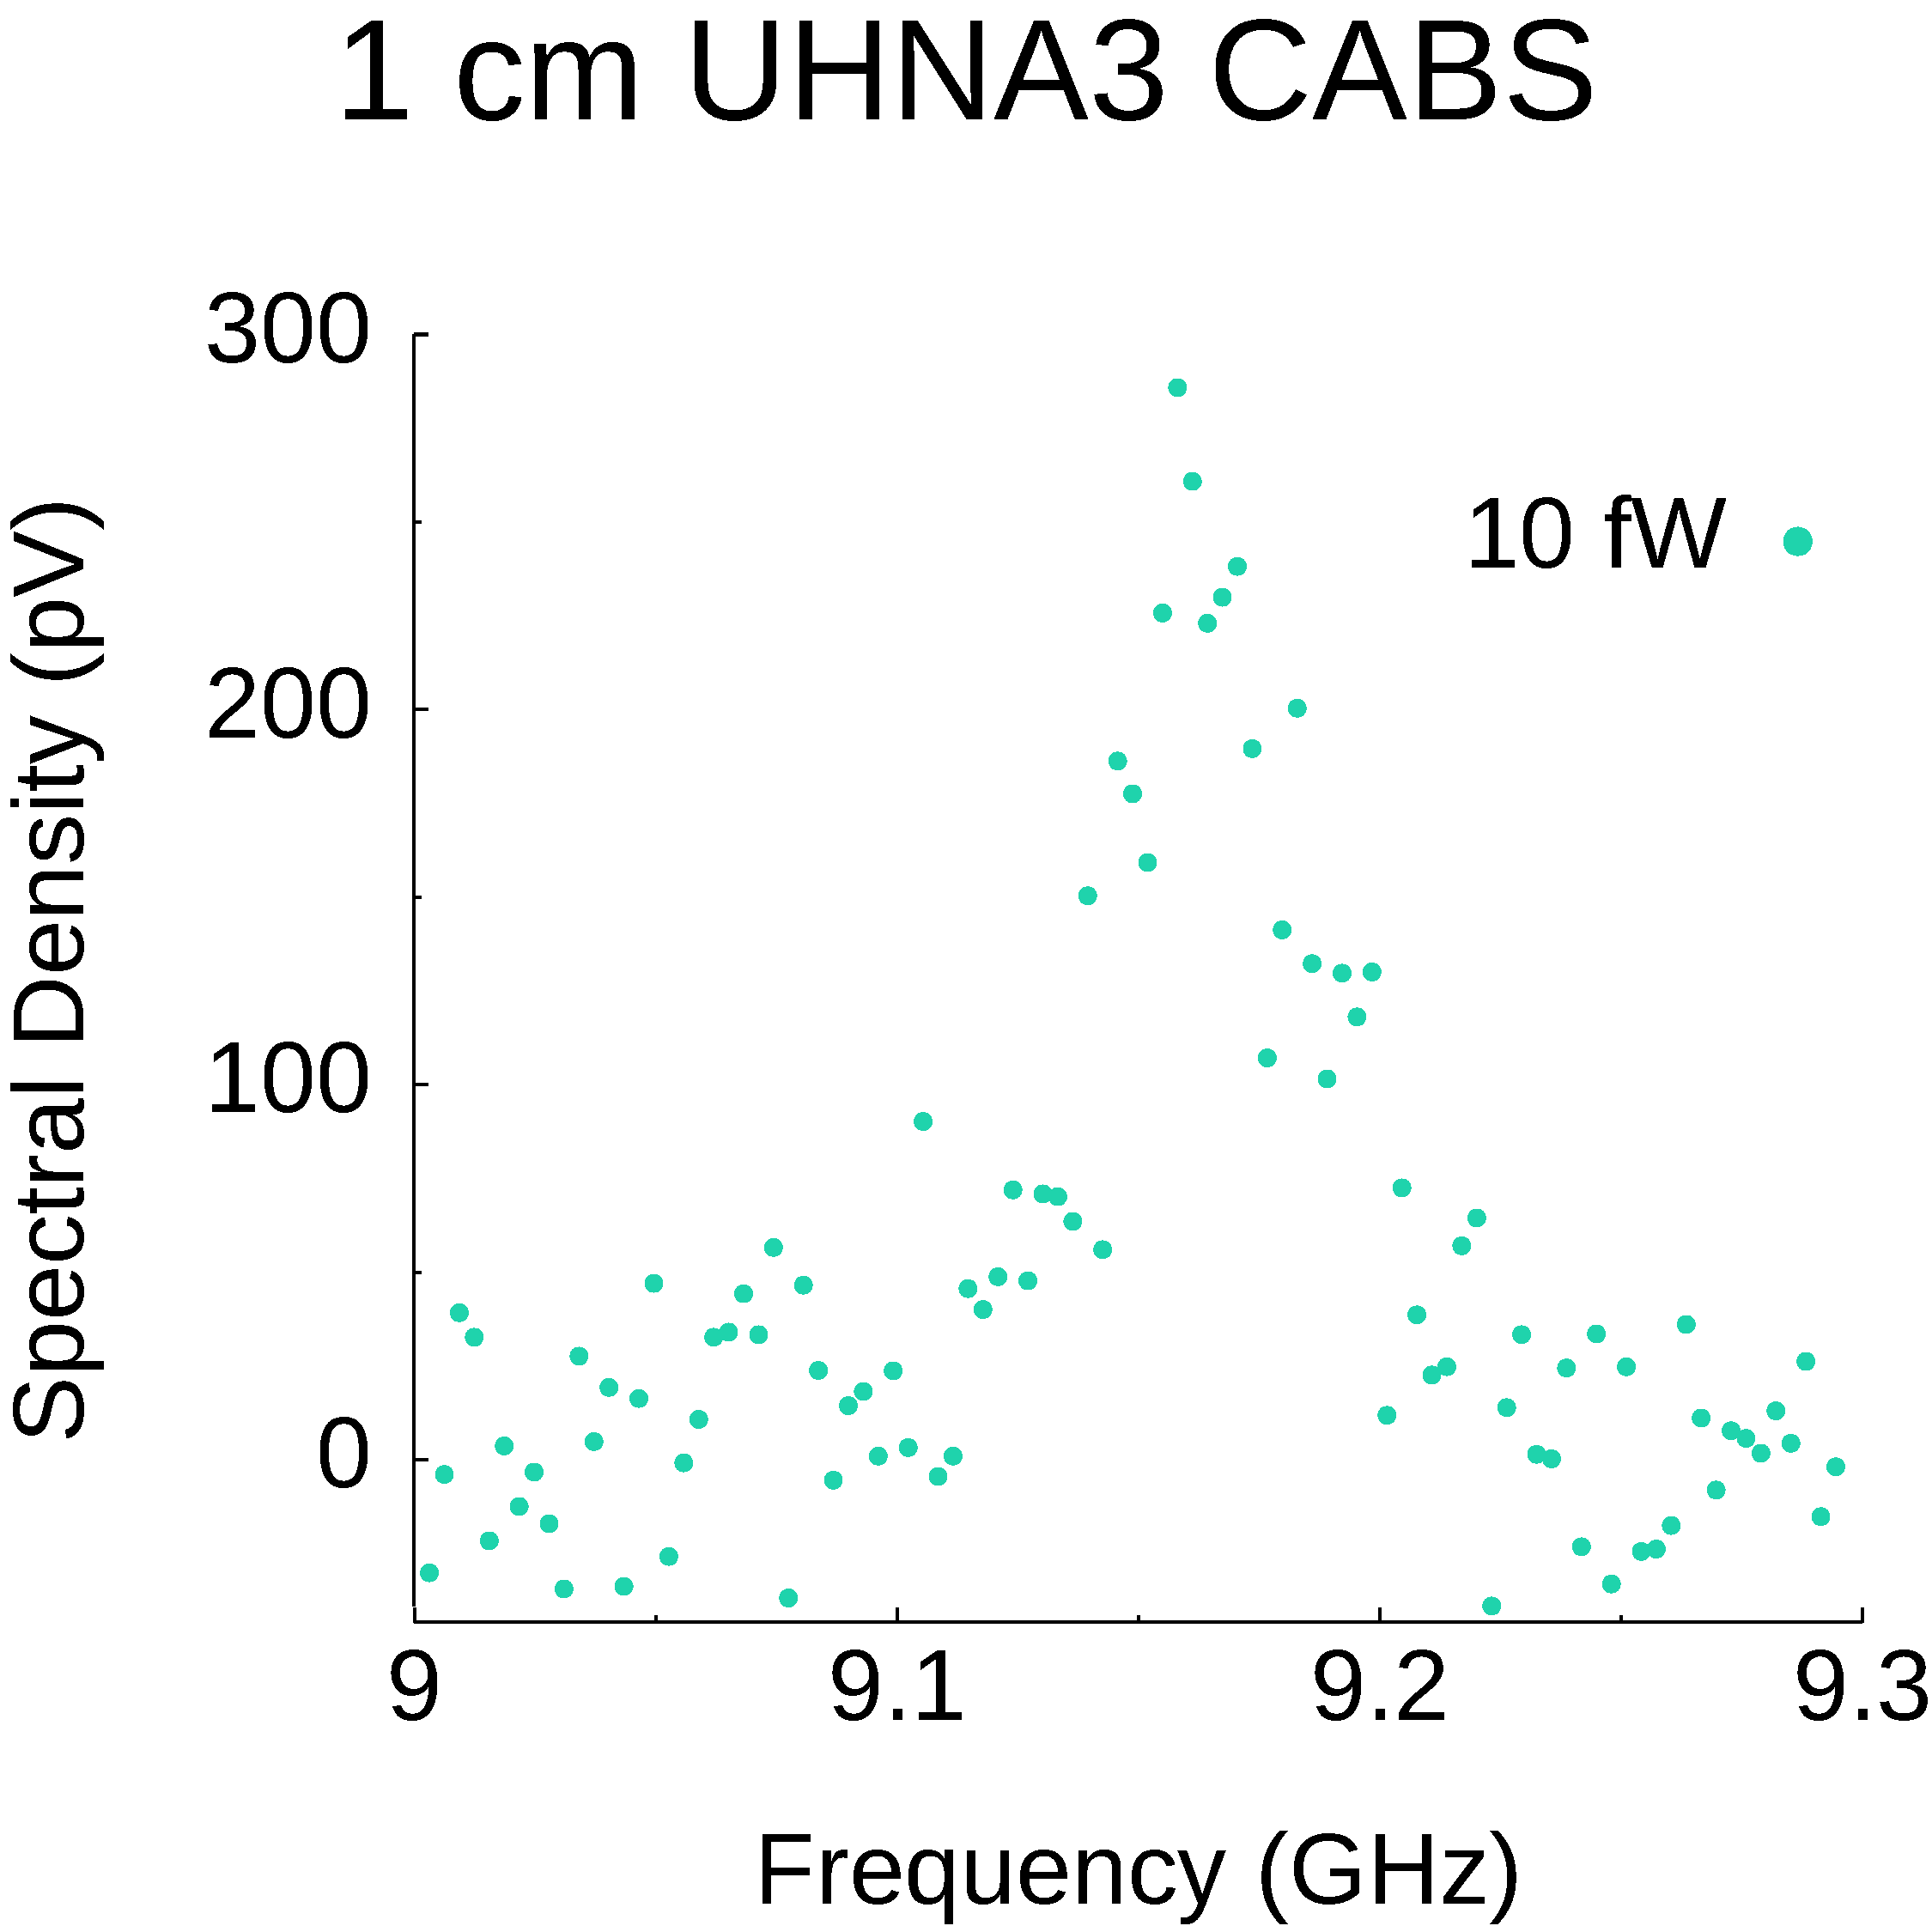
\includegraphics[width=.45\textwidth]{10fWSensitivity.pdf}
  \caption{10 fW sensitivity measurement}
  \label{fig:10fWSensitivity}
\end{figure}

We begin by testing the sensitivity of the instrument as a way of defining a performance metric for the instrument. As well, this figure will serve to inform all future measurements by indicating what material, power, and length combinations might be possible to measure. From Eq. \ref{Eq:Theoretical Framework:Scattered Power}, the sensitivity of the instrument is the minimum scattered power, $P_{Signal}$, to produce a statistically significant measurement. To determine this, we use a sample of known effective Brillouin gain, $g_{0}$, and target a specific length, $L$. We keep the pump-probe detuning, $\Delta\lambda$, constant and record the pump, Stokes, and probe optical powers to calculate the scattered power. Starting with sufficient optical powers to produce a clearly distinguishable measurement, we gradually reduce the optical powers until the sensitivity floor is reached.

We prepared a length of $1\,cm$ of Nufern's UHNA3 fiber to serve as our sensitivity testbed. The properties of UHNA3 fiber are well known and favorable for unambiguous detection of the Brillouin signal. First, it offers a Brillouin shift that is spectrally far from that of the single-mode fiber (SMF28) that constitutes much of our instrument. Additionally, due to its high germanium concentration in the core, UHNA3 fiber has a large refractive index difference between core and cladding, producing exceptionally high optical and acoustic guidance. Finally, UHNA3 fiber offers a high optomechanical nonlinear response; the Brillouin gain of UHNA3 fiber is approximately $0.6\,W^{-1}m^{-1}$ at room temperature\cite{behunin2015long}, which is about an order of magnitude larger than that of SMF28\cite{nikles1997brillouin}.

Fig. \ref{fig:10fWSensitivity} shows the Brillouin signal for a sensitivity of $P_{Signal} = [10]\,fW$. We find the signal-to-noise ratio of this measurement to be $[3]$, determined by taking the ratio of the standard errors at the peak center and completely off resonance. A standard error of $[3\sigma]$ translates to a 99.7\% confidence level in statistical significance of this measurement.


\subsection*{Measurements}
\label{Results:Measurements}

We consider two categorical samples to test the capabilities of the instrument, one fiber-coupled and one bulk material. For a fiber-coupled sample we again choose UHNA3 fiber for its higher nonlinear response. In contrast to the low-power sensitivity measurements with UHNA3 fiber, we now apply all available optical power ($\sim 1.5\,W$) to the sample to maximize the backscattered signal.

scattered power explaining why we chose 1cm length


Fig. \ref{fig:1cmUHNA3} reveals the spectral profile captured for 1 cm of UHNA3 fiber. The spectral shape is that of the expected lorentzian function, with the peak ([$9.18\,GHz$]) indicating the Brillouin resonance frequency and the FWHM ([$\sim 80\,MHz$]) indicating the dissipation rate of the fiber. [comparison to regular SBS for some measurable length of UHNA3?]

\begin{figure}[t]
  \centering
  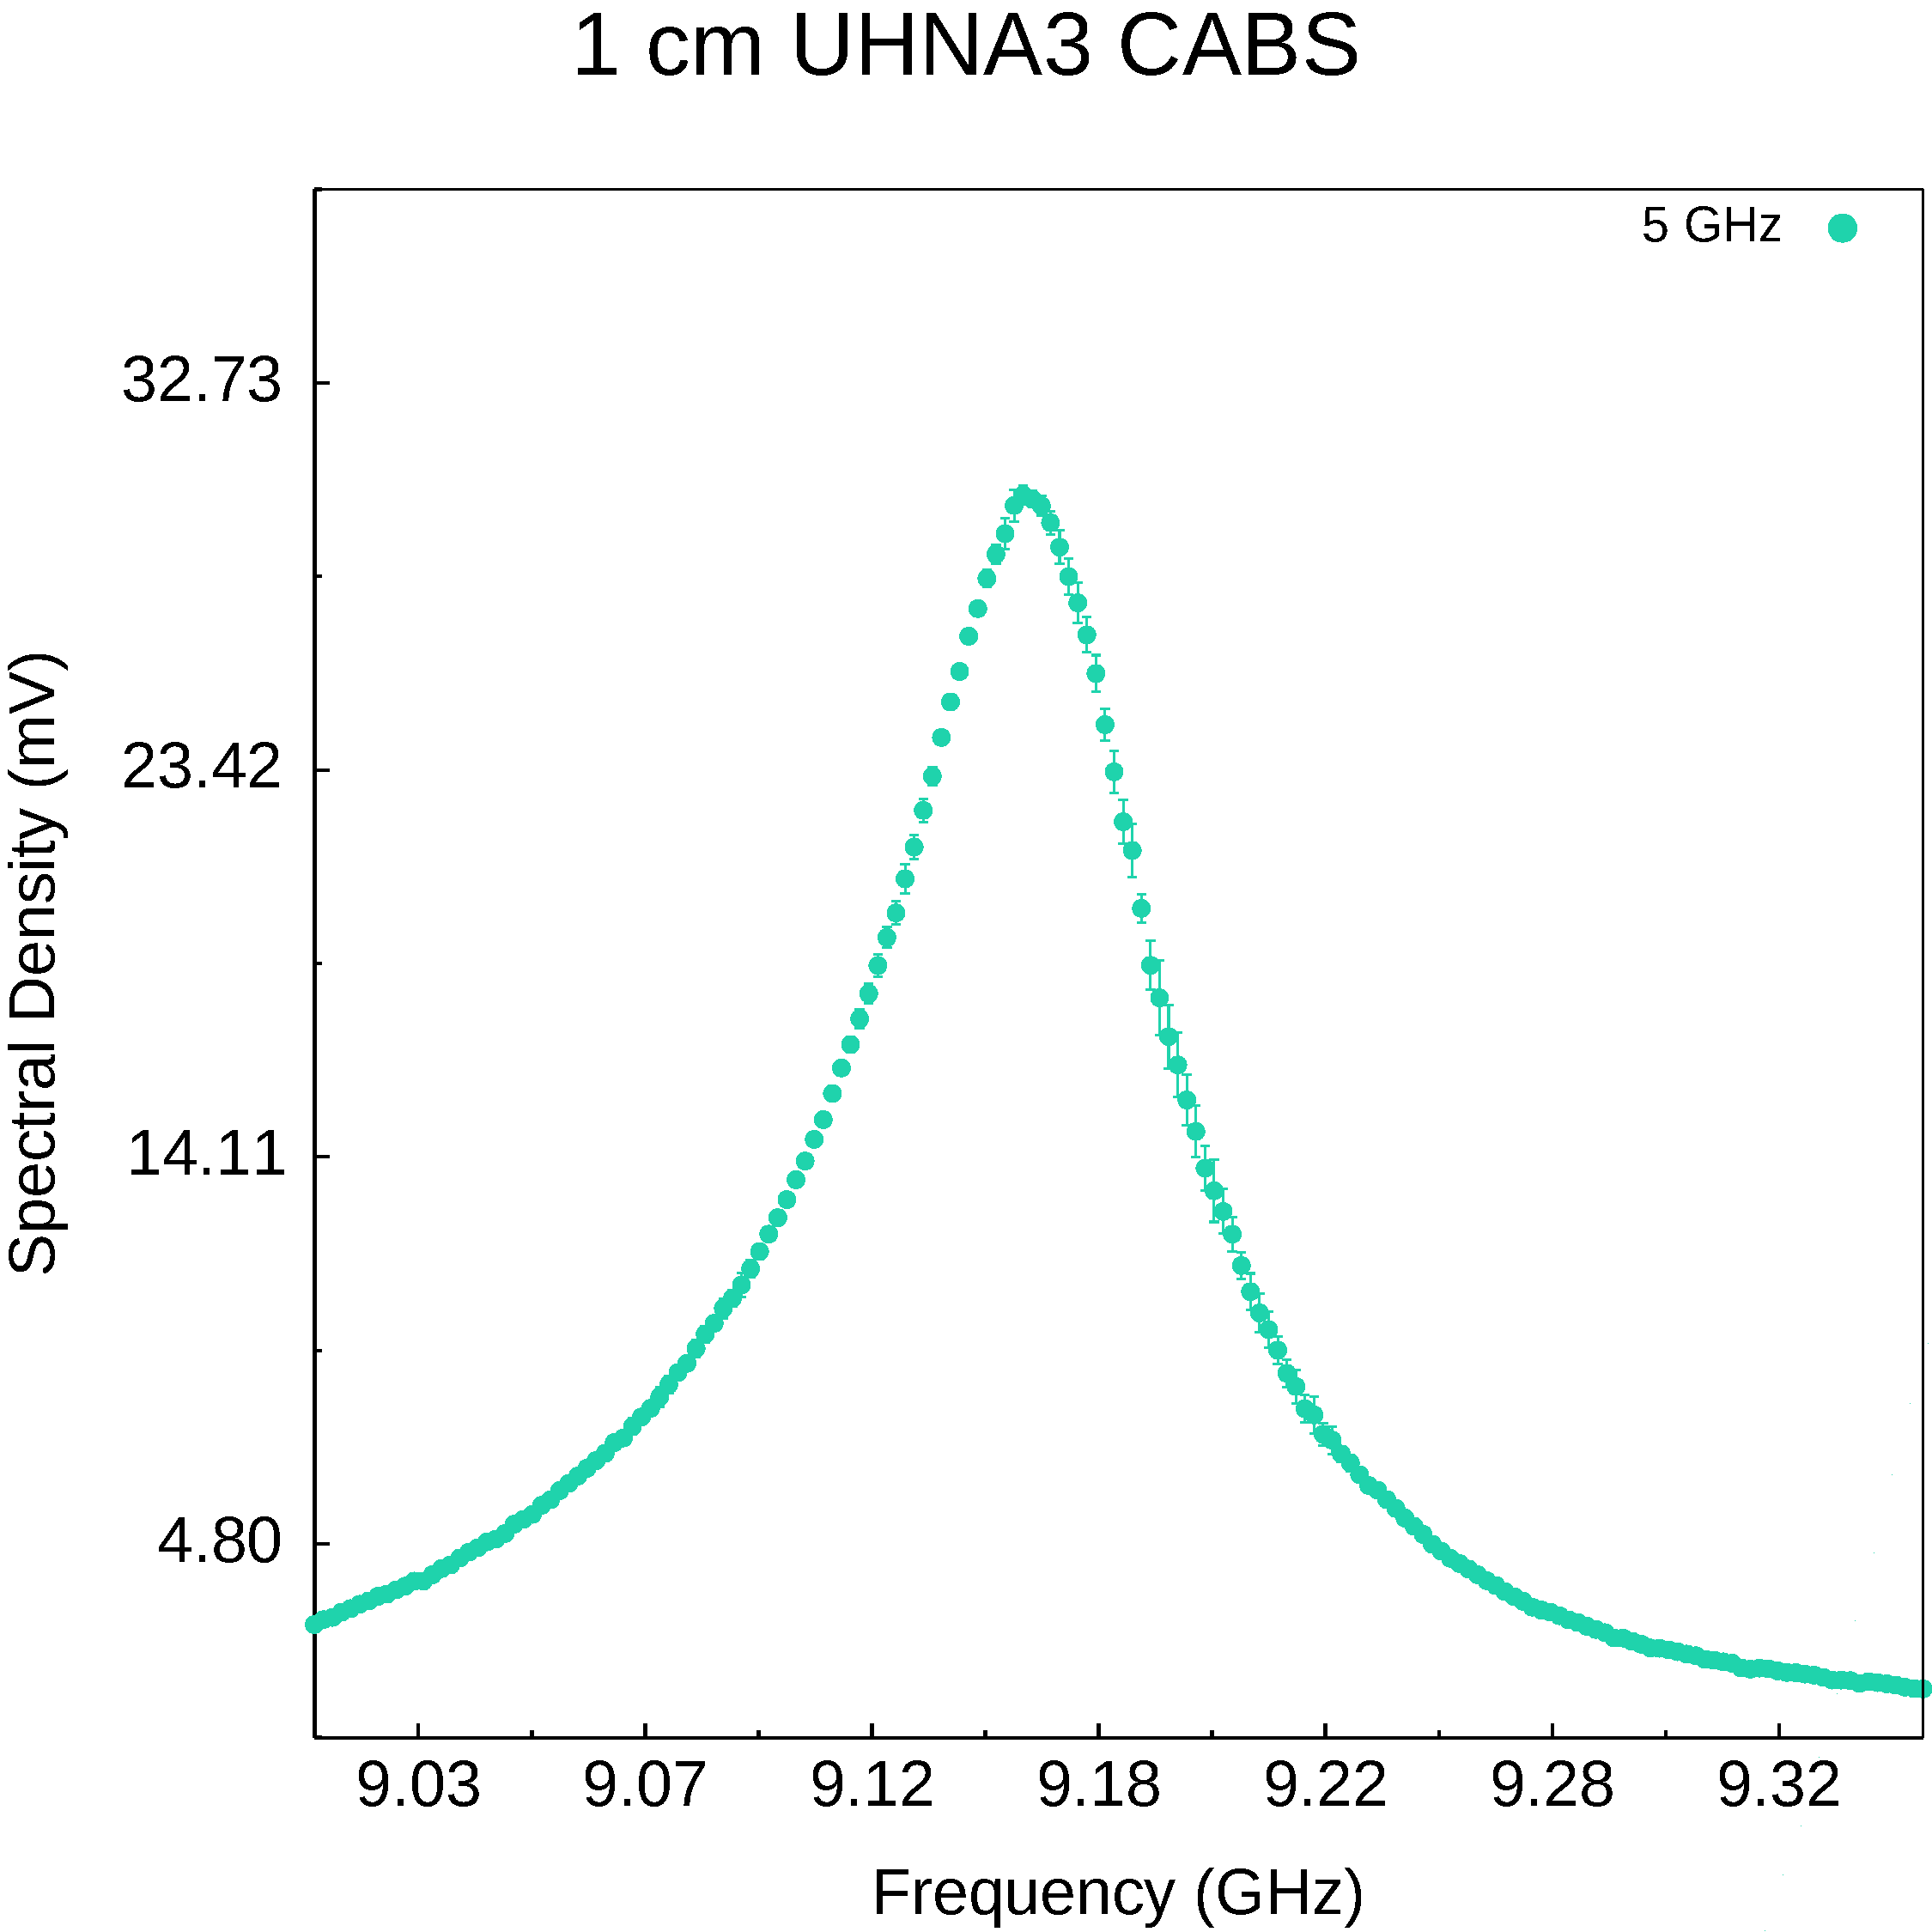
\includegraphics[width=.45\textwidth]{1cmUHNA3.pdf}
  \caption{1cm UHNA3 (fit?)}
  \label{fig:1cmUHNA3}
\end{figure}

\begin{figure}[t]
  \centering
  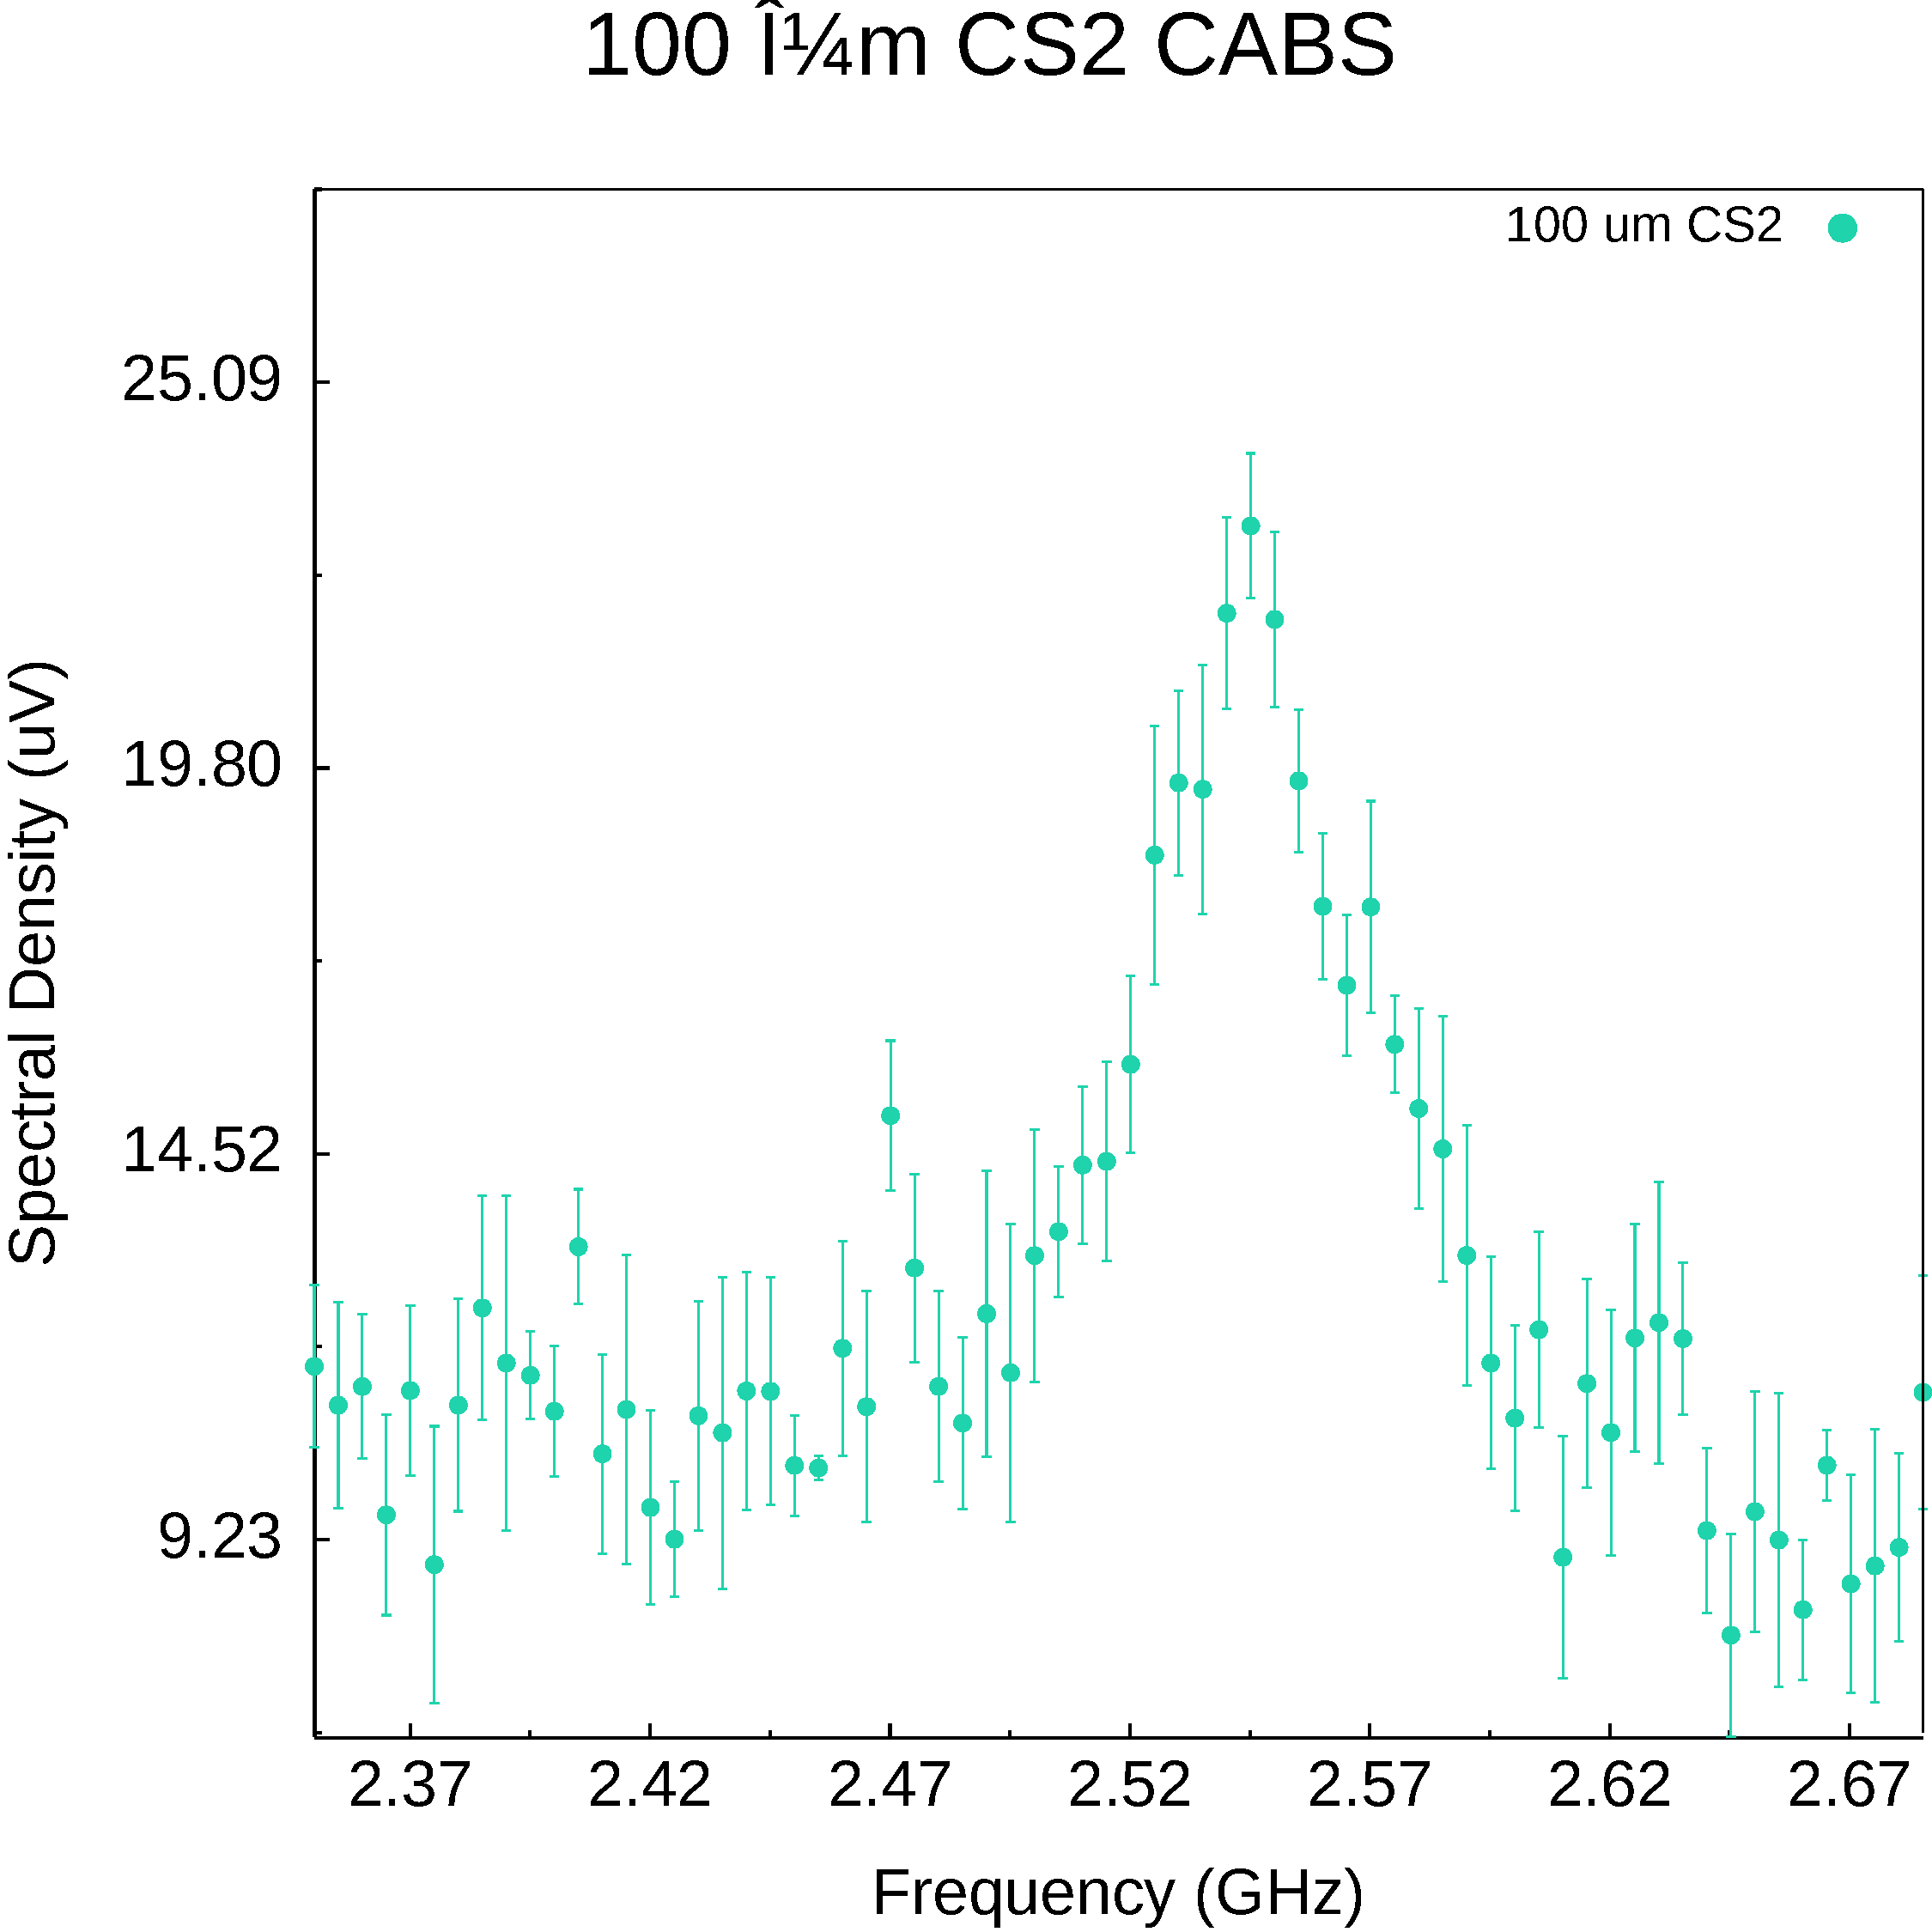
\includegraphics[width=.45\textwidth]{100umCS2.pdf}
  \caption{100um CS2}
  \label{fig:100umCS2}
\end{figure}

Fig. shows the spectral measurements achieved by the instrument, overlaid with finite-difference simulation data. In Fig. we see the expected lorentzian spectral shape in good alignment with simulation data for guided longitudinal modes in the core of the UHNA3 fiber. In Fig. , however, we see a distortion of this lorentzian shape. This is expected for partially unguided longitudinal modes, such as is the case for a bulk liquid filling the volume of a ...

Fig. \ref{fig:1cmUHNA3} shows a measurement of 1cm of UHNA3 fiber.

First, we measured Brillouin scattering in a 1-centimeter-long UHNA3 fiber at room temperature and with sub-Watt optical power (Fig. ). Figure , clearly displays the Brillouin scattering features with remarkable signal-to-noise ratio, highlighting the effectiveness of our apparatus in isolating the backscattered probe light. This observation serves as one of the main showcases of the instrument's capability.

Next, we performed Brillouin scattering measurements on a 4-millimeter-thick bulk carbon disulfide sample in a free-space optics arrangement. The observed spectrum, presented in Figure 2, exhibits well-resolved Brillouin scattering peaks. This successful measurement in a bulk sample demonstrates the versatility and adaptability of our instrument to various experimental configurations, further emphasizing the instrument's capability.

Lastly, we conducted a measurement in a 1-millimeter-long UHNA3 fiber under low-power conditions, with only 10 microwatts of power at the sample. Despite the reduced sample length and low power, the instrument's sensitivity allowed us to observe distinct Brillouin scattering features in the spectrum, as illustrated in Figure 3. This result underscores the potential of our spectrometer for nanoscale measurements and serves as a demonstration of the instrument's sensitivity, defining the sensitivity floor of the apparatus.

These three observations collectively showcase the high sensitivity, broad applicability, and impressive capabilities of our coherent stimulated phonon spectrometer in measuring Brillouin scattering across different sample types, scales, and power levels.

\begin{figure}[t]
\centering
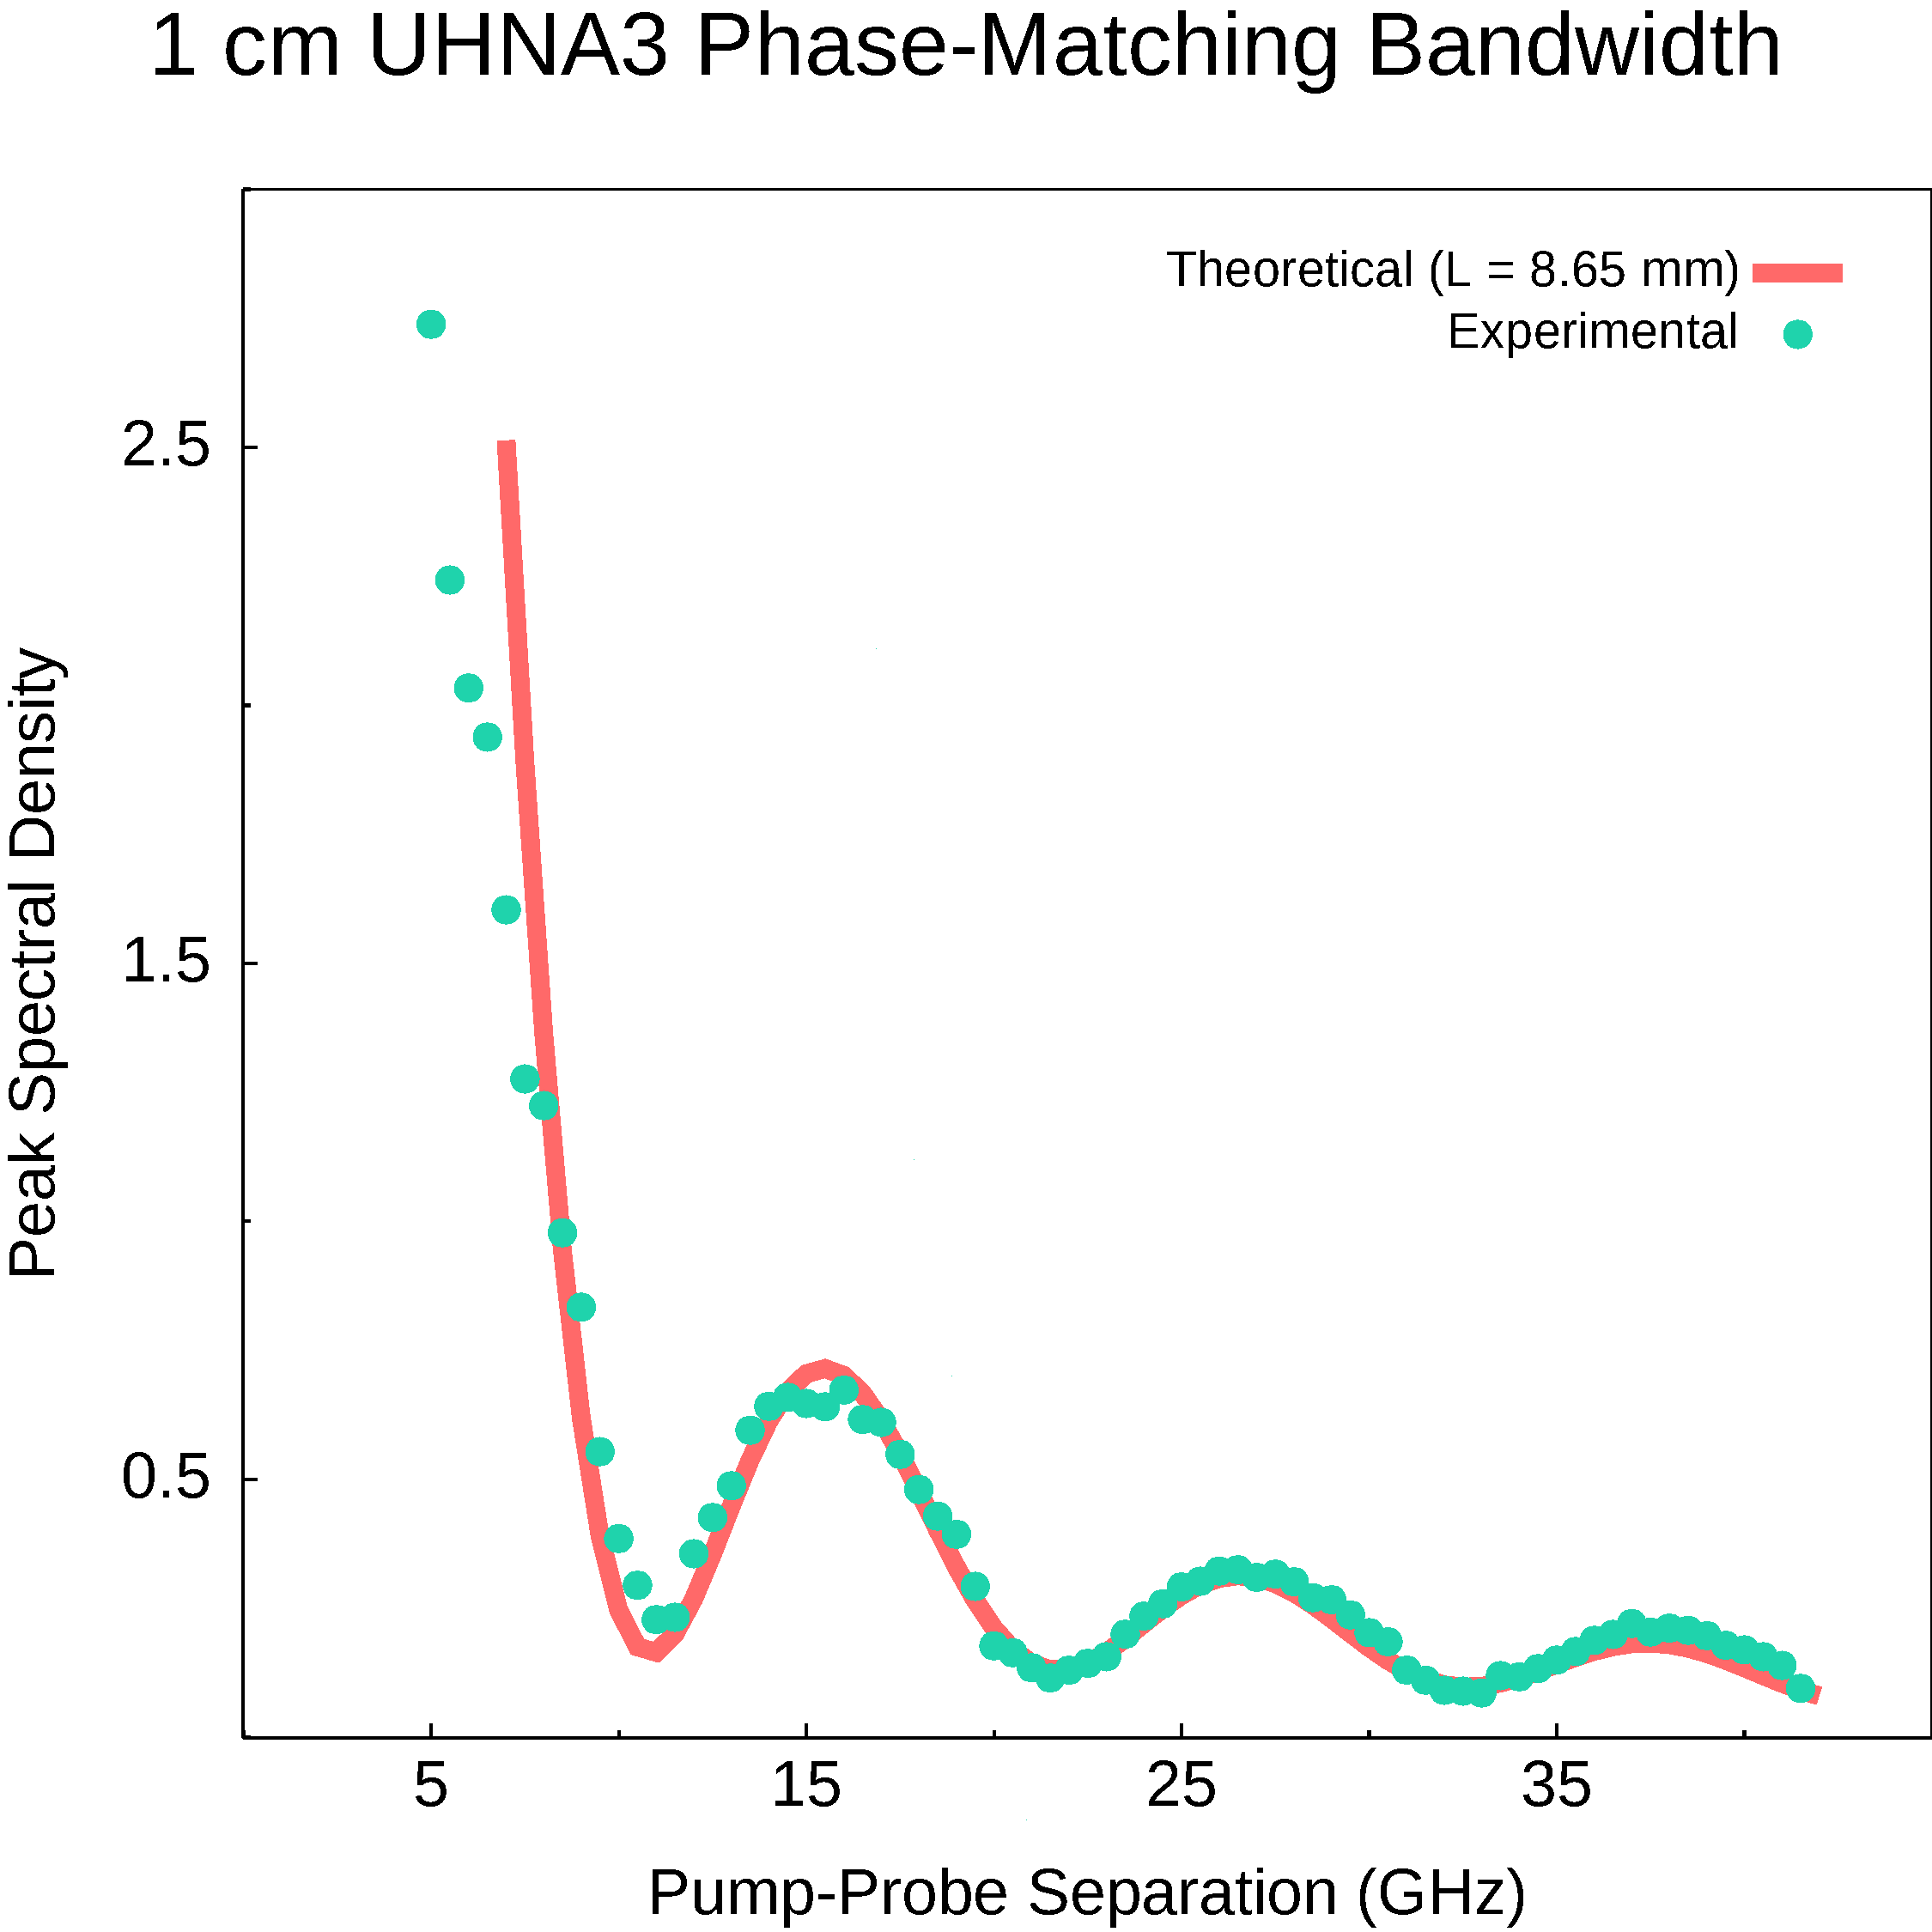
\includegraphics[width=.45\textwidth]{Phase-Match.pdf}
\caption{Phase-matching sinc func}
\label{fig:Phase-Match}
\end{figure}


\section{Discussion}
\label{Discussion}

\lipsum[1-2]


\section{Conclusion}
\label{Conclusion}

\lipsum[1]


\begin{acknowledgments}

\end{acknowledgments}

% Switch to appendices in one column
\clearpage % Ends the current page and all its floating elements.
\onecolumngrid % Switches to one-column format.

\begin{titlepage}
\centering
\vspace*{\stretch{1}}
{\Large Appendix:\\[10pt] A Coherently Stimulated Brillouin Spectrometer\par}
\vspace{\stretch{3}}
\end{titlepage}

\clearpage
\onecolumngrid

\appendix

\section{Phase Matching}
\subsection{Relaxation of Phase Matching Conditions}
\subsection{Phase Matching Bandwidth Experiments}
\subsection{Theoretical Comparison of Phase Matching Bandwidth}

\section{Coupled-Wave Equations}
\label{Appendix:Coupled-Wave Equations}

Here we derive the coupled wave equations that describe coherent stimulated Brillouin scattering involving a pump, Stokes, probe, and backscattered optical field given respectively by
\\
\begin{equation}
    \tilde{E}_{P}(z,t) = A_{P}e^{i(k_{P}z - \omega_{P}t)} + c.c.
    \label{eq:Pump optical field}
\end{equation}
\\
\begin{equation}
    \tilde{E}_{S}(z,t) = A_{S}e^{i(k_{S}z - \omega_{S}t)} + c.c.
    \label{eq:Stokes optical field}
\end{equation}
\\
\begin{equation}
    \tilde{E}_{Pr}(z,t) = A_{Pr}e^{i(k_{Pr}z - \omega_{Pr}t)} + c.c.
    \label{eq:Probe optical field}
\end{equation}
\\
\begin{equation}
    \tilde{E}_{Sig}(z,t) = A_{Sig}e^{i(k_{Sig}z - \omega_{Sig}t)} + c.c.
    \label{eq:Signal optical field}
\end{equation}
\\
\noindent and a common acoustic field given by
\\
\begin{equation}
    \tilde{\rho}(z,t) = \rho_{0} + \rho(z,t)e^{i(qz - \Omega t)} + c.c.,
    \label{eq:acoustic field}
\end{equation}
\\
\noindent where $\Omega = \omega_{P} - \omega_{S}$ and $q = k_{P} - k_{S} = 2k_{P}$.


\subsection{Acoustic Field}
\label{Coupled-Wave Equations:Acoustic Field}

As in the case of SBS \cite{boyd2020nonlinear}, we start by assuming that the material obeys the acoustic wave equation,
\\
\begin{equation}
    \frac{\partial^{2}\tilde{\rho}}{\partial t^{2}} - \Gamma^{\prime}\nabla^{2}\frac{\partial\tilde{\rho}}{\partial t} - v^{2}\nabla^{2}\tilde{\rho} = \nabla\cdot\vec{f},
    \label{eq:acoustic wave equation}
\end{equation}
\\
\noindent where $v$ is the sound speed in the material and $\Gamma^{\prime}$ is a damping parameter given by
\\
\begin{equation}
    \Gamma^{\prime} = \frac{1}{\rho}\left[\frac{4}{3}\eta_{s} + \eta_{b} + \frac{\kappa}{C_{p}}(\gamma - 1)\right],
\end{equation}
\\
\noindent where $\eta_{s}$ and $\eta_{b}$ are the shear and bulk viscosity coefficients of the material, respectively. The source term on the right side of Eq. (\ref{eq:acoustic wave equation}) is the divergence of the electrostrictive force:
\\
\begin{equation}
\begin{split}
    \vec{f} = \nabla p_{st} = \nabla \cdot \Bigg[-\frac{1}{2}\epsilon_{0}\gamma_{e}\Big(&\langle\tilde{E}_{P} \cdot \tilde{E}_{S}\rangle \\
    &+ \langle\tilde{E}_{Pr} \cdot \tilde{E}_{Sig}\rangle\Big)\Bigg],
\end{split}
\end{equation}
\\
which yields, after applying the slowly varying amplitude approximation,
\\
\begin{equation}
    \nabla\cdot\vec{f} = \epsilon_{0}\gamma_{e}q^{2}(A_{P}A_{S}^{*} + A_{Pr}A_{Sig}^{*}e^{i\Delta kz}),
\end{equation}
\\
Where $\Delta k = (k_{Pr} - k_{Sig}) - (k_{P} - k_{S})$ is the phase mismatch between the four optical fields. Only two electrostrictive terms survive terms after accounting for the orthogonal polarization of the pump and Stokes fields with respect to that of the probe and backscattered signal. Inserting this electrostrictive force term and the acoustic field (Eq. (\ref{eq:acoustic field})) into Eq. (\ref{eq:acoustic wave equation}) and assuming a slowly varying acoustic amplitude we find
\\
\begin{equation}
    -2i\Omega\frac{\partial\rho}{\partial t} - \Gamma^{\prime}2iq^{2}\Omega\rho - 2iqv^{2}\frac{\partial\rho}{\partial z} = \epsilon_{0}\gamma_{e}q^{2}(A_{P}A_{S}^{*} + A_{Pr}A_{Sig}^{*}e^{i\Delta kz}),
\end{equation}
\\
which can be restated in terms of the Brillouin linewidth, $\Gamma_{B} = q^{2}\Gamma^{\prime}$, as
\\
\begin{equation}
    -2i\Omega\frac{\partial\rho}{\partial t} - 2i\Omega\Gamma_{B}\rho - 2iqv^{2}\frac{\partial\rho}{\partial z} = \epsilon_{0}\gamma_{e}q^{2}(A_{P}A_{S}^{*} + A_{Pr}A_{Sig}^{*}e^{i\Delta kz}).
    \label{eq:in terms of Brillouin linewidth}
\end{equation}
\\
Given the phonon dispersion relations $\Omega_{B} = |q_{B}|v$ and $\Omega^{2} = q^{2}\left(v^{2} - i\Omega\Gamma^{\prime}\right)$, Eq. (\ref{eq:in terms of Brillouin linewidth}) can be rewritten as
\\
\begin{equation}
    -2i\Omega\frac{\partial\rho}{\partial t} + \left(\Omega^{2} - \Omega^{2} - i\Omega\Gamma_{B}\right)\rho - 2iqv^{2}\frac{\partial\rho}{\partial z} = \epsilon_{0}\gamma_{e}q^{2}(A_{P}A_{S}^{*} + A_{Pr}A_{Sig}^{*}e^{i\Delta kz}).
    \label{eq:in terms of Omega_B}
\end{equation}
\\
We take the common assumption that the phonon propagation distance is small compared to the distance over which the source term varies significantly, which allows the spatial derivative term in Eq. (\ref{eq:in terms of Omega_B}). We further assume steady-state conditions such that the time derivative term also vanishes, leaving
\\
\begin{equation}
    (\Omega^{2}_{B} - \Omega^{2} - i\Omega\Gamma_{B})_{\rho} = \epsilon_{0}\gamma_{e}q^{2}(A_{P}A_{S}^{*} + A_{Pr}A_{Sig}^{*}e^{i\Delta kz}).
\end{equation}
\\
We thus find the acoustic field amplitude to be
\\
\begin{equation}
    \rho(z,t) = \epsilon_{0}\gamma_{e}q^{2}\frac{A_{P}A_{S}^{*} + A_{Pr}A_{Sig}^{*}e^{i\Delta kz}}{\Omega_{B}^{2} - \Omega^{2} - i\Omega\Gamma_{B}}.
    \label{eq:Acoustic field amplitude}
\end{equation}


\subsection{Optical Fields}
\label{Coupled-Wave Equations:Optical Fields}

We now turn to the spatial evolution of the optical fields, described by the wave equation,
\\
\begin{equation}
    \frac{\partial^{2}\tilde{E}_{i}}{\partial z^{2}} - \frac{n^{2}}{c^{2}}\frac{\partial^{2}\tilde{E}_{i}}{\partial t^{2}} = \frac{1}{\epsilon_{0}c^{2}}\frac{\partial^{2}\tilde{P}_{i}}{\partial t^{2}},
    \label{eq:Wave equation}
\end{equation}
\\
where i denotes the four optical fields, namely: pump, Stokes, probe, and backscattered signal. The total nonlinear polarization that gives rise to the source term in the wave equation is given by
\\
\begin{equation}
    \tilde{P} = \epsilon_{0}\Delta\chi\tilde{E} = \epsilon_{0}\Delta\epsilon\tilde{E} = \epsilon_{0}\rho^{-1}\gamma_{e}\tilde{\rho}\tilde{E}.
\end{equation}
\\
The parts of $\tilde{P}$ that can act as phase-matched source terms for the optical fields are
\\
\begin{equation}
    \tilde{P}_{P} = p_{P}e^{i(k_{P}z - \omega_{P} t)} + c.c. = \frac{1}{2}\epsilon_{0}\rho_{0}^{-1}\gamma_{e}\rho A_{S}e^{i(k_{P}z - \omega_{P} t)}
    \label{eq:Pump phase-matched source term}
\end{equation}
\\
\begin{equation}
    \tilde{P}_{S} = p_{S}e^{i(-k_{S}z - \omega_{S} t)} + c.c. = \frac{1}{2}\epsilon_{0}\rho_{0}^{-1}\gamma_{e}\rho^{*} A_{P}e^{i(-k_{S}z - \omega_{S} t)}
    \label{eq:Stokes phase-matched source term}
\end{equation}
\\
\begin{equation}
    \tilde{P}_{Pr} = p_{Pr}e^{i(k_{Pr}z - \omega_{Pr} t)} + c.c. = \frac{1}{2}\epsilon_{0}\rho_{0}^{-1}\gamma_{e}\rho A_{Sig}e^{i(k_{Pr}z - \omega_{Pr} t)}e^{i\Delta kz}
    \label{eq:Probe phase-matched source term}
\end{equation}
\\
\begin{equation}
    \tilde{P}_{Sig} = p_{Sig}e^{i(-k_{Sig}z - \omega_{Sig} t)} + c.c. = \frac{1}{2}\epsilon_{0}\rho_{0}^{-1}\gamma_{e}\rho^{*} A_{Pr}e^{i(-k_{Sig}z - \omega_{Sig} t)}e^{-i\Delta kz}.
    \label{eq:Signal phase-matched source term}
\end{equation}
\\
Inserting the optical fields (Eqs. \ref{eq:Pump optical field}-\ref{eq:Signal optical field}) and phase-matched source terms (Eqs. \ref{eq:Pump phase-matched source term}-\ref{eq:Signal phase-matched source term}) into Eq. (\ref{eq:Wave equation}), we obtain
\\
\begin{equation}
    \frac{\partial A_{P}}{\partial z} + \frac{n}{c}\frac{\partial A_{P}}{\partial t} = \frac{i\omega_{P}\gamma_{e}}{2nc\rho_{0}}\rho A_{2}
\end{equation}
\\
\begin{equation}
    -\frac{\partial A_{S}}{\partial z} + \frac{n}{c}\frac{\partial A_{S}}{\partial t} = \frac{i\omega_{S}\gamma_{e}}{2nc\rho_{0}}\rho^{*}A_{P}
\end{equation}
\\
\begin{equation}
    \frac{\partial A_{Pr}}{\partial z} + \frac{n}{c}\frac{\partial A_{Pr}}{\partial t} = \frac{i\omega_{Pr}\gamma_{e}}{2nc\rho_{0}}\rho A_{Sig}
\end{equation}
\\
\begin{equation}
    -\frac{\partial A_{Sig}}{\partial z} + \frac{n}{c}\frac{\partial A_{Sig}}{\partial t} = \frac{i\omega_{Sig}\gamma_{e}}{2nc\rho_{0}}\rho^{*}A_{Pr}
\end{equation}
\\
We again assume steady-state conditions, allowing the time derivative term to be dropped. Plugging in the acoustic field amplitude (Eq. \ref{eq:Acoustic field amplitude}), we arrive at the coupled-amplitude wave equations for the optical fields,
\\
\begin{equation}
    \frac{\partial A_{P}}{\partial z} = \frac{i\epsilon_{0}\omega_{P} q^{2}\gamma_{e}^{2}}{2nc\rho_{0}}\frac{A_{P}|A_{S}|^{2} + A_{Pr}A_{Sig}^{*}A_{S}e^{i\Delta kz}}{\Omega_{B}^{2} - \Omega^{2} - i\Omega\Gamma_{B}}
\end{equation}
\\
\begin{equation}
    \frac{\partial A_{S}}{\partial z} = -\frac{i\epsilon_{0}\omega_{S} q^{2}\gamma_{e}^{2}}{2nc\rho_{0}}\frac{|A_{P}|^{2}A_{S}^{*} + A_{Pr}A_{Sig}^{*}A_{P}e^{-i\Delta kz}}{\Omega_{B}^{2} - \Omega^{2} - i\Omega\Gamma_{B}}
\end{equation}
\\
\begin{equation}
    \frac{\partial A_{Pr}}{\partial z} = \frac{i\epsilon_{0}\omega_{Pr} q^{2}\gamma_{e}^{2}}{2nc\rho_{0}}\frac{A_{P}A_{S}^{*}A_{Sig} + A_{Pr}|A_{Sig}|^{2}e^{i\Delta kz}}{\Omega_{B}^{2} - \Omega^{2} - i\Omega\Gamma_{B}}
\end{equation}
\\
\begin{equation}
    \frac{\partial A_{Sig}}{\partial z} = -\frac{i\epsilon_{0}\omega_{Sig} q^{2}\gamma_{e}^{2}}{2nc\rho_{0}}\frac{A_{P}A_{S}^{*}A_{Pr} + |A_{Pr}|^{2}A_{Sig}^{*}e^{-i\Delta kz}}{\Omega_{B}^{2} - \Omega^{2} - i\Omega\Gamma_{B}}
    \label{eq:Signal coupled-amplitude wave equation}
\end{equation}
\\
Integrating Eq. \ref{eq:Signal coupled-amplitude wave equation} along the effective length gives the amplitudes of each optical field,
\\
\begin{equation}
  A_{P} = \frac{i\epsilon_{0}\omega_{P}q^{2}\gamma_{e}^{2}}{2nc\rho_{0}}\frac{A_{P}|A_{S}|^{2} + A_{Pr}A_{Sig}^{*}A_{S}}{\Omega_{B}^{2}-\Omega^{2}-i\Omega\Gamma_{B}} \frac{e^{i\Delta kL}-1}{i\Delta k},
\end{equation}
\\
\begin{equation}
  A_{S} = -\frac{i\epsilon_{0}\omega_{S}q^{2}\gamma_{e}^{2}}{2nc\rho_{0}}\frac{|A_{P}|^{2}A_{S}^{*} + A_{Pr}A_{Sig}^{*}A_{P}}{\Omega_{B}^{2}-\Omega^{2}-i\Omega\Gamma_{B}} \frac{e^{-i\Delta kL}-1}{-i\Delta k},
\end{equation}
\\
\begin{equation}
  A_{Pr} = \frac{i\epsilon_{0}\omega_{Pr}q^{2}\gamma_{e}^{2}}{2nc\rho_{0}}\frac{A_{P}A_{S}^{*}A_{Sig} + A_{Pr}|A_{Sig}|^{2}}{\Omega_{B}^{2}-\Omega^{2}-i\Omega\Gamma_{B}} \frac{e^{i\Delta kL}-1}{i\Delta k},
\end{equation}
\\
\begin{equation}
  A_{Sig} = -\frac{i\epsilon_{0}\omega_{Sig}q^{2}\gamma_{e}^{2}}{2nc\rho_{0}}\frac{A_{P}A_{S}^{*}A_{Pr} + |A_{Pr}|^{2}A_{Sig}^{*}}{\Omega_{B}^{2}-\Omega^{2}-i\Omega\Gamma_{B}} \frac{e^{-i\Delta kL}-1}{-i\Delta k}.
\end{equation}
\\
The intensity of the backscattered signal is given by the magnitude of the time-averaged Poynting vector, given by
\\
\begin{equation}
  I_{i} = 2n_{i}\epsilon_{0}c|A_{i}|^{2}, \qquad i = 1,2,3,
\end{equation}
\\
which gives
\\
\begin{equation}
  I_{Sig} = \frac{\epsilon_{0}^{2}\omega^{2}q^{4}\gamma_{e}^{4}}{4n^{2}c^{2}\rho_{0}^{2}}\frac{|A_{P}|^{2}|A_{S}|^{2}|A_{Pr}|^{2}}{(\Omega_{B} - \Omega)^{4} - \Omega^{2}\Gamma_{B}^{2}}\bigg|\frac{e^{-i\Delta kL} - 1}{-i\Delta k}\bigg|^{2}.
\end{equation}
\\
Here we have taken the real part and dropped the very small terms containing the signal amplitude. The squared modulus term containing $\Delta k$ can be reduced as
\\
\begin{gather}
  \bigg|\frac{e^{-i\Delta kL} - 1}{-i\Delta k}\bigg|^{2} = \frac{(e^{-i\Delta kL} - 1)(e^{i\Delta kL} - 1)}{(\Delta k)^{2}} = \frac{L^{2}}{(\Delta kL)^{2}}\Bigg[ 2 - 2\Bigg(\frac{e^{i\Delta kL} + e^{-1\Delta kL}}{2}\Bigg)\Bigg] \notag \\ \notag \\
  = \frac{2L^{2}(1 - cos\Delta kL)}{(\Delta kL)^{2}} = \frac{4L^{2}sin^{2}\big(\frac{\Delta kL}{2}\big)}{\big(\Delta kL\big)^{2}} = \frac{L^{2}sin^{2}\big(\frac{\Delta kL}{2}\big)}{\big(\frac{\Delta kL}{2}\big)^{2}} = L^{2}sinc^{2}\bigg(\frac{\Delta kL}{2}\bigg)
\end{gather}
\\
and the optical fields can be written in terms of the intensities to produce the backscattered intensity of the signal:
\\
\begin{equation}
  I_{Sig} = \frac{\epsilon_{0}^{2}\omega^{2}q^{4}\gamma_{e}^{4}}{4n^{2}c^{2}\rho_{0}^{2}}\frac{I_{P}I_{S}I_{Pr}}{(\Omega_{B} - \Omega)^{4} - \Omega^{2}\Gamma_{B}^{2}}L^{2}sinc^{2}\left(\frac{\Delta kL}{2}\right).
\end{equation}
\\
Defining the intensities as $I_{i} = 2n\epsilon_{0}cA_{i}A_{i}^{*}$, the backscattered signal intensity is reduced to [see green writing to far right in onenote coupled wave equations of CABS]

To find the power of the backscattered signal, we would integrate this intensity over the effective area. Approximated for fiber as $\pi r^{2}$ where r is the effective mode field diameter, this becomes
\\
\begin{equation}
  P_{Sig} = \pi r^{2}\frac{\epsilon_{0}^{2}\omega^{2}q^{4}\gamma_{e}^{4}}{4n^{2}c^{2}\rho_{0}^{2}}\frac{P_{P}P_{S}P_{Pr}}{(\Omega_{B} - \Omega)^{4} - \Omega^{2}\Gamma_{B}^{2}}L^{2}sinc^{2}\left(\frac{\Delta kL}{2}\right).
\end{equation}
\newpage

\section{Instrument Details}
\subsection{List of Salient Components}
\subsection{Laser Output: Whisper Mode vs. Dither Mode}
\subsection{Lock-in Settings}

\section{Experimental Techniques}
\subsection{Background Subtraction: Probe Off, Sample In}
\subsection{Background Subtraction: Probe On, Sample Out}
\subsection{Polarization Control Limit}
\subsection{Pump, Stokes, Probe Polarization Optimization}
\subsection{Local Oscillator Polarization Optimization}
\subsection{Lock-in Detector Settings}
\subsection{Detection Bandwidth}

\section{Pump, Stokes, and Probe Contribute Equally}

\section{Comparison to SBS}
\subsection{1 Centimeter UHNA3 Scattered Power}
\subsection{100 Micrometers CS2 Scattered Power}

\section{Measurement Theory}
\subsection{Heterodyne Detection}
\subsection{Lock-in Detection}

\section{Sensitivity}
\subsection{Sensitivity Measurements}
\subsection{Current Sensitivity Limitors}
\subsection{Ultimate Sensitivity Limitor: Shot Noise}

\section{Alternative Configurations}
\subsection{Mirrored Design}
\subsection{Radial Acoustic Modes}
\subsection{Shear Acoustic Modes}
\subsection{Coherent Anti-Stokes Raman Spectrometer}

\twocolumngrid

\bibliography{apssamp}% Produces the bibliography via BibTeX.

\end{document}
%
% ****** End of file apssamp.tex ******
